\chapter{State of the Art\label{cha:chapter2}}

\section{HTTP Adaptive Streaming\label{sec:live}}

For more than 15 years HTTP adaptive streaming (HAS) has been the defacto standard media streaming protocol with the release of HTTP live streaming (HLS) \footnote{HLS for Developer: \url{https://developer.apple.com/streaming/}} in 2009 \cite{rfc8216} and subsequently in 2012 \footnote{DASH First ISO Standard: \url{https://www.iso.org/standard/57623.html}} with the release Dynamic adaptive streaming over HTTP (DASH).

In both of the protocols a media stream is split into a number of different representations, each being a transcode of the original stream with different quality levels or in case of audio and subtitles they can also represent different languages. Each of these representations inturn has its media stream split into small chunks. These chunks enable the media players to dynamically switch the currently playing representations to adapt to the current situation, they also enable separation of the acquisition of the stream into many individual HTTP requests instead of downloading the entire stream in one go.

Both of these protocols make use of a manifest to give the media player all relevant information to acquire the media stream. In case of DASH this manifest is the Media Presentation Description (MPD). It uses the file ending \texttt{.mpd}. This MPD is an XML \cite{rfc5364} file which contains every detail about one specific media stream. In contrast to this approach, HLS splits this information into one Master Playlist and separate Media Playlists. These files use the file ending \texttt{.m3u8}. They are encoded as plain text UTF-8 \cite{rfc3629} files with a proprietary method of encoding the contained information. The Master Playlist contains information about the individual representations, as well the references to the Media Playlists each of which corresponds one specific representation. 

The MPD and Master Playlist act as the entry points of their respective media stream and are used to initialize a media player to play that stream. The players download these files and use the contained information to play the media stream. While the media is playing the players analyze the current streaming situation and based on a number of parameters, like network conditions, buffer level, playing quality, available qualities, etc. use an adaptive bitrate (ABR) algorithm whether or not to switch to a different quality to ensure smooth playback.

\section{C2PA\label{c2pa}}

As previously mentioned the goal of C2PA is the creation of a tamper-proof method of embedding metadata into media. This metadata is supposed to contain all information relevant in the creation of said media as well as all the editing steps applied to it. Ultimately, this data encodes the provenance of media to provide transparency, knowledge and the trust in it.

The technical specifications of C2PA detail the motivations, goals and methodologies. These specifications are currently on version 2.2 \footnote{C2PA Technical Specification v2.2: \url{https://c2pa.org/specifications/specifications/2.2/specs/C2PA_Specification.html}}, however, when I started this thesis the C2PA implementation this work is based on was still on version 2.0, thus I will be referencing version 2.0 for everything related to the technical specifications \footnote{C2PA Technical Specification v2.0: \url{https://c2pa.org/specifications/specifications/2.0/specs/C2PA_Specification.html}}. Everything in this section is referenced to this technical specification unless denoted otherwise.

Here I give an example of what an ideally integrated lifecycle of media content would look like. A photographer takes an image using a camera. This camera has integrated C2PA capabilities and would embed C2PA metadata into the image. This metadata would contain information like the location where the image was taken, model name of the camera, camera settings, like ISO values, zoom level, used to take the image, EXIF data, credentials of the photographer who took the image, automatic processing steps applied by the camera and possibly any additional data the camera was configured to include. The photographer then takes this image to an editor who further edits this image with software. This program is also integrated with C2PA capabilities and would extended the already embedded C2PA metadata with information about the editing process. This additional data could included information about color corrections, lighting changes, cropping, removal and addition of objects, application of filters, credentials from the editor and any other image manipulations applied to the image. The image is now ready for publication. It is uploaded to social media and these services often apply modifications to media during upload, like compression to make them more portable, conversion to a different data type or other steps. These are naturally also C2PA integrated and they further extend the C2PA metadata by including the processing formation, service that applied the changes and so on. The image is now viewable by everyone on the respective platforms. The websites and programs displaying this image are integrated with C2PA validation tools and verify that the image hasn't been tampered with by validating the C2PA metadata. They then indicate that the image is trustworthy and also provide the option for users to look at the metadata.

\subsection{Assertion}

An \texttt{Assertion} encapsulates a piece of information about the media asset. It is created during the signing process. Assertions are an integral part of the C2PA Manifest. Each Assertion is identified by an unique label. There are predefined labels and Assertion data but it is also possible to include any type of proprietary data as Assertion. 

An example of a predefined Assertion follows in \Cref{sec:bmff_assertion}.

\subsection{Claim}

The \texttt{Claim} reference all Assertions of the C2PA Manifest they are contained in. It is digitally signed and tamper-proof. The Claim is also an integral part of the C2PA Manifest.

\subsection{Claim Signature}

The \texttt{Claim Signature} is the final part of the C2PA Manifest and it it is the digital signature of the Claim.

\subsection{C2PA Manifest}

The \texttt{C2PA Manifest} (or just Manifest) contains the three aforementioned parts: the Claim Signature, the Claim and the Assertions. Each Manifest contains one Claim Signature, one Claim and a set of Assertions. They are contained in the Manifest Store of an media asset.

\subsection{Manifest Store}

The C2PA metadata is wrapped in the \texttt{Manifest Store}. A Manifest Store contains all C2PA Manifests. The last of these Manifests is the so called Active Manifests, which is the most recently added Manifests and it contains the credentials that are verifiable. The Manifest Store can be either directly embedded into the media asset or it can be referenced in the asset as external.

An example of how a Manifest Store can look like can be seen in \Cref{fig:manifest_store}.

\begin{figure}
    \centering
    \includegraphics[scale=0.3]{manifest-store.pdf}
    \caption{Example Manifest Store \cite{manifestStore}}
    \label{fig:manifest_store}
\end{figure}

\subsection{BMFF Hash Assertion\label{sec:bmff_assertion}}

The BMFF Hash Assertion (label: \texttt{c2pa.hash.bmff}) is the C2PA Data Hash \footnote{Data Hash: \url{https://c2pa.org/specifications/specifications/2.0/specs/C2PA_Specification.html\#_data_hash}} Assertion embedded in fragmented BMFF media files and is required in these files for validation. This Assertion is encapsulated by the Rust data structure \texttt{BmffHash}, see \Cref{code:bmff_hash}. It contains the exclusion ranges used to create the data hashes of the fragmented files (struct field \texttt{exclusions}), the name of hashing algorithm used (struct field \texttt{alg}), the data hash, as byte buffer, of the corresponding file (struct field \texttt{hash} / this field is not used for BMFF media which is split into multiple files, this use case of the thesis), the Merkle Trees (struct field \texttt{merkle}) and the BMFF hashing version used (struct field \texttt{bmff\_version}).

The Merkle Trees are described by an array of the Rust data structure \texttt{MerkleMap}, see \Cref{code:merkle_map}. Each Merkle Tree contains its unique ID (struct field \texttt{unique\_id}), its local ID (struct field \texttt{local\_id}), the number of leaves in this tree (struct field \texttt{count}), the name of the hashing algorithm used (struct field \texttt{alg}), the data hash of the initialization fragment, as byte buffer and the layer of the Merkle Tree stored for reference, more on that later, as array of byte buffer (struct field \texttt{hashes}).

\begin{minipage}{0.95\linewidth}
\begin{lstlisting}[caption={BmffHash Rust Definition}, label=code:bmff_hash, language=Rust, captionpos=b]
    pub struct BmmfHash {
        // the exclusion ranges
        exclusions: Vec<ExclusionMap>,
        // name of the hashing algorithm
        alg: Option<String>,
        // the data hash
        hash: Option<ByteBuf>,
        // the Merkle Tree
        merkle: Option<Vec<MerkleMap>>,
        // name of the assertion
        name: Option<String>,
        // deprecated beginning with BMFF Version 2
        url: Option<UriT>,
        // BMFF Version, here 2
        bmff_version: usize,
    }
\end{lstlisting}
\end{minipage}

\begin{minipage}{0.95\linewidth}
\begin{lstlisting}[caption={MerkleMap Rust Definition}, label=code:merkle_map, language=Rust, captionpos=b]
    pub struct MerkleMap {
        // unique ID
        pub unique:id: u32,
        // local ID
        pub local_id: u32,
        // number of leave
        pub count: u32,
        // name of hashing algorithm
        pub alg: Option<String>,
        // hash of initialization fragment
        pub init_hash: Option<ByteBuf>,
        // Merkle Tree reference layer
        pub hashes: VecByteBuf,
    }
\end{lstlisting}
\end{minipage}

\subsubsection{BMFF-Based Hashing}

The hashing of BMFF-based data has certain requirements set by the specifications that need to be followed. All the data of a BMFF file must be included in the hashing data, except specific parts as defined by the \texttt{ExclusionMap} list. These exclusions are included in the corresponding Assertion, \texttt{BmffHash} in this case, as mention in the preceding section.

The data structure of an exclusion is details in \Cref{code:exclusion_map}. It contains one mandatory field \texttt{xpath}, which describes the path to the corresponding BMFF Box, similar to a file system path, using the BMFF Box names in \texttt{4cc} notation. When a specific BMFF Box occurs multiple times they can be addressed by their index using array notation and positive non-zero indices. The remaining data fields are all optional. When all fields are left out, the BMFF Box specified by \texttt{xpath} is to be excluded in its entirety. The next field is \texttt{length} which denotes the length a BMFF Box must have to be excluded from the hash, including the box header. The \texttt{data} field is a list of \texttt{DataMap} type, which holds an byte offset and a data value, if the BMFF Box contains the exact data value at the specified offset it is to be excluded from the hash. The \texttt{subset} data field allows exclusion of specific data ranges. It is a list of \texttt{SubsetMap}, which encapsulates a byte offset and a length. Data is excluded from the hash starting at the offset for the specified length. The offsets in the list must monotonically increasing and no subset must overlap with another. The final entry can have a length of \texttt{0} to indicate to exclude the remainder of the BMFF Box. The length can also exceed the BMFF Box boundary to achieve the same as length \texttt{0}. The field \texttt{version} indicates to exclude the BMFF Box if it has this version, this can only be set for BMFF Boxes which are FullBoxes. The \texttt{flags} is a byte string of exactly three bytes and if the BMFF Box has these flags set it must be excluded. This can also only be applied to FullBoxes. The final field \texttt{exact} is a boolean and can only be set if \texttt{flags} is also set and indicates whether the flags must match exactly to exclude the BMFF Box from the hash. Otherwise the flags must have at least the same bits set and additional flags can also be set. If \texttt{exact} if not set it defaults to \texttt{true}.

\begin{minipage}{0.95\linewidth}
\begin{lstlisting}[caption={ExclusionMap Rust Definition}, label=code:exclusion_map, language=Rust, captionpos=b]
    pub struct ExclusionMap {
        // path to the BMFF Box
        pub xpath: String,
        // exclude if box has this exact length
        pub length: Option<u32>,
        // exclude when exact data is contained
        pub data: Option<Vec<DataMap>>,
        // exclude specific data ranges
        pub subset: Option<Vec<SubsetMap>>,
        // exclude if the BMFF Box has this version
        pub version: Option<u8>,
        // exclude if these flags are set
        pub flags: Option<ByteBuf>,
        // exclude if flags match exactly
        pub exact: Option<bool>,
    }
\end{lstlisting}
\end{minipage}

In case the C2PA Manifest is embedded directly into an BMFF file, the BMFF Box it is contained in must be excluded from the hash.

When a BMFF Box is removed after the C2PA Manifest has been created, it should be replaced with a \texttt{"free"} BMFF Box with the same length to make sure the hash is not invalidated by the removal of the Box. If the removal of a Box is expected to happen, the effected Box shall be replaced by a \texttt{"free"} BMFF Box of the same size for the duration of the signing. The placeholder must then be excluded from the hash. Once the signing is completed the Box needs to be put back in its original place.

Since adding C2PA Manifest into BMFF-based file via MP4 boxes changes the positions of these Box, the position of root BMFF Box needs to be included in the hash to ensure the correct placement of Boxes.

\subsubsection{Merkle Tree\label{sec:merkle}}

A Merkle Tree can be used to create a signature of a large dataset by fragmenting it into smaller pieces. Then it is possible to validate one of these pieces as part of the whole dataset without needing to have access to the entire dataset. The C2PA specifications use a Merkle Tree for fragmented BMFF media.

A Merkle Tree is a binary tree that is built from the bottom up. The first row are the leaves of the Merkle Tree. The leaves are the fragmented pieces of the dataset, in this case the media segments, more specifically they are the hashes of the data. The next row contains the parents of the previous row's nodes. If a parent node has both left and right children then the data hash of the parent node is the hash of the two children hashes concatenated, otherwise the children node hash is copied. This is repeated until the row with only a single node has been reached, this node is the root of the Merkle Tree \cite{merkle}.

Once the Merkle Tree is fully built only one of the layers has to be kept in memory or stored in a data structure, I am calling this the \texttt{reference tree layer} from here on. Which layer is used for this, is up to the application. The weight between number of hashes stored and number of steps required for validation has to be considered for choosing the which layer to keep, the higher the layer used, the smaller this layer but the more nodes, the proof hashes, are needed to validate individual fragments. These proof hashes are assigned to each leaf. The proofs are hashes that are part of the full Merkle Tree and they are the hashes are required to validate a leaf. They are the sibling nodes along the path from the leaf up to the reference tree layer.

A simple example of this can be seen in \Cref{fig:merkle_example}. For example the hash \texttt{H3} is the resulting hash of the concatenation of fragment hashes \texttt{F5} and \texttt{F6}, while the hash \texttt{H9} is the result using the hashes \texttt{H6} and \texttt{H7}. The fragment hash \texttt{F11} and hash \texttt{H8} are examples of the case where there is one child missing and that node is simply copied. In this example hash \texttt{H10} is the root of the Merkle Tree.

\begin{figure}
    \centering
    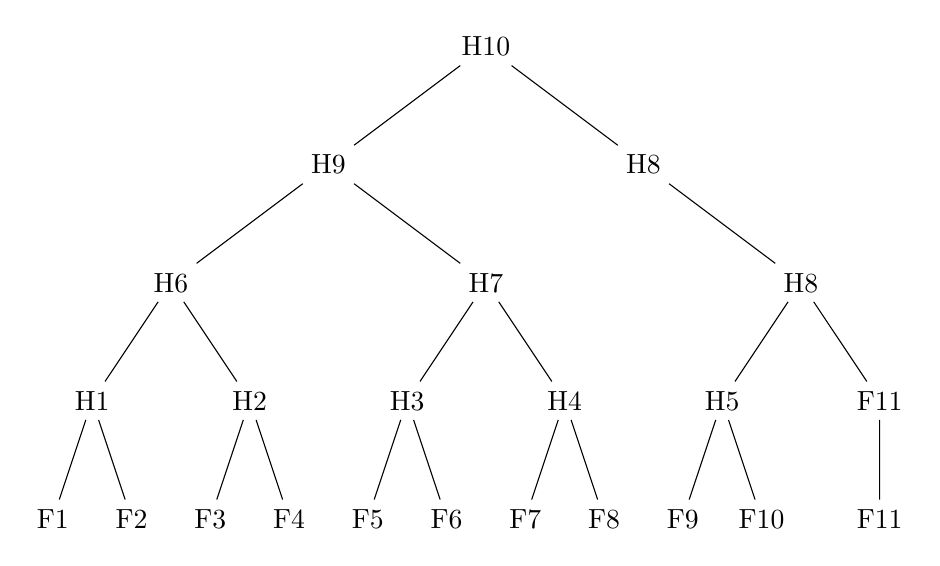
\begin{tikzpicture}[level distance=1.5cm,
        level 1/.style={sibling distance=4cm},
        level 2/.style={sibling distance=4cm},
        level 3/.style={sibling distance=2cm},
        level 4/.style={sibling distance=1cm},
        ]
        \node { H10 }
            child { node { H9 }
                child { node { H6 }
                    child { node { H1 } 
                        child { node { F1 } }
                        child { node { F2 } }
                    }
                    child { node { H2 } 
                        child { node { F3 } }
                        child { node { F4 } }
                    }
                }
                child { node { H7 }
                    child { node { H3 } 
                        child { node { F5 } }
                        child { node { F6 } }
                    }
                    child { node { H4 } 
                        child { node { F7 } }
                        child { node { F8 } }
                    }
                }
            }
            child { node { H8 }
                child [missing]
                child { node { H8 }
                    child { node { H5 } 
                        child { node { F9 } }
                        child { node { F10 } }
                    }
                    child { node { F11 } 
                        child { node { F11 } }
                    }
                }
            };
    \end{tikzpicture}
    \caption{Simple Merkle Tree Example}
    \label{fig:merkle_example}
\end{figure}

\subsubsection{Validation}

The validation can be either performed only on the initialization fragment or on at least one fragment in conjunction with the initialization fragment.

The initialization segment contains the C2PA manifest packaged in a \texttt{uuid} BMFF box. In a fragmented BMFF context this manifest must contains the aforementioned \texttt{c2pa.hash.bmff} Assertion. To verify the initialization segment one has to read the C2PA manifest and use the included hash exclusion ranges to recreate the hash of the initialization segment. If this hash is equal to the one found in the manifest then the initialization segment is validated as trustworthy.

Each fragment also contains a \texttt{uuid} box. However, the fragments only contain a CBOR-encoded \cite{rfc8949} data structure which holds information required for validation: the proof \texttt{hashes}, the \texttt{local\_id} and \texttt{unique\_id} and the \texttt{location} on that particular Merkle Tree, shown by the Rust structure BmffMerkleMap in \Cref{code:bmff_merkle}. The two IDs are required to identify the corresponding Merkle Tree from the C2PA manifest in the initialization segment and the location is the leaf index of the fragment which is needed to determine whether this fragment is the left or right child of their parent node.

\begin{minipage}{0.95\linewidth}
\begin{lstlisting}[caption={BmffMerkleMap Rust Definition}, label=code:bmff_merkle, language=Rust, captionpos=b]
    pub struct BmffMerkleMap {
        // unique ID
        pub unique_id: u32,
        // local ID
        pub local_id: u32,
        // leave index on the Merkle Tree
        pub location: u32,
        // proof hashes
        pub hashes: Option<VecByteBuf>,
    }
\end{lstlisting}
\end{minipage}

The validation of a fragment requires the successful validation of the accompanying initialization segment. First step of the validation is calculation of the data hash using the exclusion ranges according to the C2PA manifest. Next the proofs are used in sequence to reconstruct the Merkle Tree. This is done by first determining whether the fragment is a left or right node. The \texttt{location} values begin at zero indicating that an even \texttt{location} representing a left node and an odd \texttt{location} a right node. The first proof is the direct sibling of the fragment. Then the first parent can be calculated using the first proof and the information of \texttt{location} by concatenating the two hashes (left + right) and hashing the result again using the algorithm specified in the C2PA manifest. This is repeated with the newly created hash and the next proof until all proofs have been used. The final hash resulting from these steps should equal one of the hashes located in the corresponding Merkle Tree from the C2PA manifest. If that is the case the fragment has been validated as trustworthy \footnote{BMFF-Based Hash Validation: \url{https://c2pa.org/specifications/specifications/2.0/specs/C2PA_Specification.html\#_validation}}. A simplified version of the can be seen in pseudo code in \Cref{alg:validate}.

\begin{algorithm}[H]
    \begin{algorithmic}[1]
        \Require $refTreeLayer$ \Comment{read from C2PA Manifest}
        \Require $location$ \Comment{read from Fragment}
        \State $fragHash \gets hash(fragment)$
        \ForAll{$proof \gets fragment.proofs$}
            \If{location is right}
                \State $fragHash \gets hash(proof + fragHash)$
            \Else
                \State $fragHash \gets hash(fragHash + proof)$
            \EndIf
        \EndFor
        \If{fragHash in refTreeLayer}
            \State fragment is valid
        \Else
            \State fragment is invalid
        \EndIf
    \end{algorithmic}
    \caption{Validating a Fragment}
    \label{alg:validate}
\end{algorithm}

\subsection{Signing Fragmented BMFF Files\label{sec:sign_bmff}}

As previously mentioned, in the context of a fragment MP4 video, the initialization segment file contains the \texttt{"uuid"} BMFF Box with the Manifest Store and each corresponding media fragment contains a \texttt{"uuid"} BMFF Box with the CBOR-encoded \texttt{BmffMerkleMap}.

Currently, the signing process if only defined for VoD content. It requires in full set of media fragments and the initialization fragment. The BMFF-specific parts of the signing process starts with the creation of a placeholder Merkle Tree based on the number of media fragments. In the next step the fragments all receive a preliminary \texttt{BmffMerkleMap} embedded into their \texttt{"uuid"} BMFF Box, it contains the final values for the two ID fields and the location but the hashes are only placeholder data. Now that the media fragments have the embedded \texttt{"uuid"} BMFF Box, they are ready to be hashed. These hashes can now be used to generate the final Merkle Tree and this inturn can be used to insert the correct proof hashes in the media fragments. Now any of the rows of the Merkle Tree can be added into the \texttt{MerkleMap} alongside a placeholder hash of the initialization fragment. This preliminary data is now inserted into the initialization fragment, which is now ready to be hashed. This hash replaces the previously set placeholder.

\section{Concurrent Approaches}

\todo[inline]{DRM?}
\todo[inline]{Fingerprinting?}
\todo[inline]{Watermarking?}
\todo[inline]{other live pocs}